\documentclass[10pt]{scrreprt}
\usepackage[a4paper, top=30mm, left=25mm, right=25mm, bottom=30mm]{geometry}
\usepackage[utf8]{inputenc}

\usepackage[Bjornstrup]{fncychap}
\usepackage{ngerman}
\usepackage{graphicx}
\usepackage{epstopdf}
\usepackage{etoolbox}
\usepackage{enumitem}
\usepackage{url}
\usepackage{numprint}
\usepackage{longtable}
\usepackage{tabu}
\usepackage{multirow}
\usepackage{caption}
\usepackage{array}
\usepackage{amssymb}
\usepackage{makeidx}
\makeindex



\makeatletter
\patchcmd{\@makechapterhead}{\vspace*{50\p@}}{\vspace*{-20\p@}}{}{}
\patchcmd{\@makeschapterhead}{\vspace*{50\p@}}{\vspace*{7\p@}}{}{}
\patchcmd{\DOTIS}{\vskip 40\p@}{\vskip -12\p@} 
\makeatother
  
\captionsetup[figure]{labelfont={sf,bf},textfont={sf}}
\deffootnotemark{[\thefootnotemark]}
\deffootnote{1.5em}{1em}{[\thefootnotemark] }
\setlength{\parindent}{0pt}
\renewcommand{\labelitemi}{ \raisebox{0.3ex}{\small$\blacktriangleright$} }
\renewcommand{\labelitemii}{ \raisebox{0.3ex}{\small$\triangleright$} }

\newcommand{\sfbf}[1]{\textbf{\sffamily #1}}
\newcommand{\sfit}[1]{\textit{\sffamily #1}}
\newcommand{\W}{\sfbf{W}}
\newcommand{\ziellabel}{Z}
\newcommand{\JoglEarth}{\raisebox{-1.2mm}{
\includegraphics[scale=0.33]{Logo-Text.eps}} }
\newcommand{\textref}[1]{\mbox{\raisebox{0.1ex}{\small$\rightarrow$ }\textit{#1}}}

\newenvironment{details}[1][6pt]{%
  \parskip#1 \parindent6mm \raggedright%
  \def\item{\par\ignorespaces\hangindent=5mm \hangafter1}}{%
  \par\ignorespaces} 

\begin{document}

\thispagestyle{empty}
\sffamily
 
\title{Handbuch}

\begin{figure}
\begin{flushright}
	
\includegraphics[scale=0.4]{uniLogo.eps}
\vspace{2.0 cm}
\end{flushright}
\end{figure}

\begin{center}
\vspace{2.0 cm}
{\LARGE SEP – Wintersemester 2013/14}

\vspace{1.0 cm}
\textbf{{\Huge Handbuch}}

\vspace{0.4 cm}
\begin{figure}[!htb]
\begin{center}
	
\includegraphics[scale=1.5]{Logo-Print.eps}
\end{center}
\end{figure}

\vspace{0.2 cm}
\textbf{{\huge OpenStreetMap: Die Welt in 3D}}

\vspace{1.5 cm}
03.12.2013

\vspace{0.5 cm}
Version: 1.0

\vspace{1.5 cm}
{\Large Projektbetreuer: Peter Barth}

\end{center}


\pagebreak
\rmfamily
\tableofcontents


\chapter{Vorwort}
\section*{Ziel \& Zweck}
Dieses Handbuch soll Ihnen als umfassendes Nachschlagewerk zur Bedienung von \JoglEarth dienen. 

\vspace{3mm}
Die ausführlichen Beschreibungen der Abläufe inklusive der Übungsaufgaben sollen das Arbeiten mit der vorliegenden Software erleichtern. 

\vspace{3mm}
\section*{Übungsaufgaben}
Das Lösen der Übungen soll Ihnen die Möglichkeit bieten, die Bedienung von \JoglEarth zu verinnerlichen.

\vspace{3mm}
\section*{Tipps \& Tricks}
Sie erhalten verschiedenste Tipps \& Tricks - die mittels spezieller Symbole gekennzeichnet sind - um effizient mit der Anwendung arbeiten zu können, wie im nachfolgenden Kapitel \textit{\textref Zur Benutzung dieses Handbuchs} beschrieben.

\vspace{3mm}
\section*{Entwicklerteam}
Das Entwicklerteam bestehend aus
\begin{itemize}
\item Christof Blauberger
\item Thomas Eder
\item Gabriele Haas
\item Fabian Knorr
\item Sebastian Reichl
\item Constantin Wenger
\end{itemize}
hat hoffentlich Ihre Neugierde für \textit{'die Welt in 3D'} geweckt.\\
Viel Spaß bei der Nutzung von \JoglEarth. 



\chapter{Zur Benutzung dieses Handbuchs}

\section*{Hinweise und Symbole}
Im vorliegenden Handbuch werden wichtige Begriffe hervorgehoben.\\

Die folgende Formatierungen sind im Handbuch zu finden:

\begin{center}
\begin{tabular}{|>{\centering \arraybackslash}m{3cm}|m{10cm}|}
\hline 
\rule[-1ex]{0pt}{3ex} \textbf{Formatierung} & \textbf{Erläuterung} \\
\hline
\hline
\rule[-1ex]{0pt}{4ex} \textit{kursiv} &   \\
\hline
\rule[-1ex]{0pt}{4ex} \textbf{fett} &   \\
\hline
\rule[-1ex]{0pt}{4ex} \underline{unterstrichen} &  \\
\hline
\end{tabular}
\end{center}


\vspace{3mm}
Es werden im Handbuch einige Symbole verwendet, welche die Arbeit mit dem Handbuch erleichtern sollen:

\begin{center}
\begin{tabular}{|>{\centering \arraybackslash}m{3cm}|m{10cm}|}
\hline 
\rule[-1ex]{0pt}{3ex}\textbf{Symbol} & \textbf{Erläuterung} \\ 
\hline
\hline
\rule[-1ex]{0pt}{6ex}
\includegraphics[scale=0.5]{images/info.eps} & Tipps \& Tricks  \\ 
\hline
\rule[-1ex]{0pt}{6ex}
\includegraphics[scale=0.5]{images/quest.eps} & Übungen \\
\hline
\rule[-1ex]{0pt}{3ex} \textref Kap. & Hinweis auf ein weiterführendes Kapitel im Handbuch \\
\hline
\end{tabular}
\end{center}


\vspace{3mm}
Die im Handbuch abgebildeten Screenshots können vom \JoglEarth Erscheinungsbild auf Ihrem PC abweichen, was durch das jeweils verwendete Betriebssystem bedingt ist. Die Funktionalitäten und Anordnungen der Schaltflächen sind jedoch unter allen Betriebssystemen identisch. Die in diesem Handbuch abgebildeten Screenshots wurden teilweise unter Windows und teilweise unter Linux erstellt.\\

Der Inhalt des Handbuchs beschränkt sich zur Erleichterung der Lektüre auf die Erklärung der wesentlichsten Programmfunktionen.\\





\chapter{Allgemeines}
\section{Ausgangssituation}
Die Karten des OpenStreetMap-Projekts erfreuen sich immer größerer Beliebtheit. Der Detailgrad, die Menge an verschiedenen Merkmalen und die Genauigkeit der Daten sind denen ihrer Konkurrenz in den meisten Regionen der Welt weit voraus. Durch die große Auswahl an Informationen und die Flexibilität in der Darstellung eröffnen sich unzählige Anwendungsmöglichkeiten.

\vspace{0.5cm}
Die Projektion einer Straßenkarte auf einen dreidimensionalen Globus ist die intuitivste und geographisch korrekteste Darstellung. Bei \JoglEarth wurden folgende Schwerpunkte gesetzt:
\begin{itemize}
\item Verwendung der freien Kartendaten des OpenStreetMap-Projekts
\item Realisierung einer dreidimensionalen Globusoberfläche mit den Höhendaten der NASA
\item Intuitive Bedienung der Anwendung ohne Einarbeitungszeit
\item Die Möglichkeit der spielerischen Benutzung durch Kinder ohne nennenswerte PC-Kenntnisse
\item Vollständige Plattformunabhängigkeit durch Java
\item Effiziente Speicher- und Bandbreitennutzung
\end{itemize}


\vspace{2mm}
\section{Anwendungsbereich}
\JoglEarth bietet eine dreidimensionale Ansicht der Welt sowie eine ebene Kartenansicht. Beides erfolgt auf Basis des OpenStreetMap-Projekts und den Satellitendaten der NASA. \\

Die grafische Benutzeroberfläche zeigt dafür im dreidimensionalen Modus eine Weltkugel, die frei gedreht und gezoomt werden kann, und im zweidimensionalen einen Ausschnitt der Weltkarte. Die Karte kann aus verschiedenen Kategorien wie Satellitenbildern oder Straßenkarten gewählt werden. Die Steuerung erfolgt mit Tastatur und Maus. \\

Mit einer Suchfunktion kann im Umkreis oder global nach Orten gesucht werden. Punkte besonderen Interesses wie Gaststätten oder Banken können über dem Kartenbild eingeblendet werden.


\vspace{3mm}
\section{Zielgruppe}
Primäre Zielgruppe des Systems sind Privatanwender, die eine andere Art der Kartendarstellung als die der typischen Onlinekarten bevorzugen. \\

Auch soll die Anwendung wissbegierige Kinder ansprechen. Voraussetzung ist lediglich der geübte Umgang mit der Maus und/ oder Tastatur.





\chapter{Systemvoraussetzungen}
\section{Software}
Da das Projekt auf Java setzt, ist es betriebssystemunabhängig. Es muss lediglich das Java Runtime Environment (JRE) in Version 7 sowie ein Fenstersystem und Netzwerkunterstützung zur Verfügung stehen. Um dieses Handbuch über die Hilfefunktion anzeigen zu können, muss auf dem System außerdem ein PDF-Betrachter installiert sein. Zusätzliche Programmbibliotheken, die zum Ausführen des Softwarepakets nötig sind, wurden mitgeliefert.\\

Folgende Konfigurationen sollen mindestens unterstützt werden:
\begin{itemize}
\item Windows 7 und 8 auf x86{\_}64 mit den Herstellertreibern von nVidia und AMD
\item Linux auf x86{\_}64 mit X.org und proprietären Treibern von nVidia / AMD sowie den freien radeon-Treibern für AMD
\end{itemize}

\vspace{3mm}
\section{Hardware}
Wie schon bei der Software der Fall sollte die Anwendung auch mit nahezu allen modernen Desktopsystemen kompatibel sein. Folgende (oder eine gleichwertige) Konfiguration wird jedoch für ein optimales Benutzererlebnis mindestens empfohlen:
\begin{itemize}
\item Dual-Core-Prozessor mit 1 GHz Taktfrequenz
\item 2 Gigabyte RAM
\item 200 Megabyte freier Speicherplatz
\item Grafikkarte: Onboard-Grafik mit OpenGL 2.0-Unterstützung
\item Bildschirm mit 1024x768 Pixeln Auflösung und 24 Bit Farbtiefe
\item Standard-Tastatur und Maus
\end{itemize}

\vspace{3mm}
\section{Orgware}
Zum Laden der Kartendaten wird eine durchgehende Internetverbindung benötigt. Um die Wartezeiten akzeptabel zu halten wird mindestens 1MBit/s empfohlen.





\chapter{Erste Schritte}


\section{Starten von JoglEarth}
%Öffnen der JAR, Jogl-Earth
%Screenshot vom USB-Stick-Dateiverzeichnis?
%Einstiegsfenster, Erklärung vom Ansichts-, Orte-, Einstellungstab inkl. Screenshot

Nach dem Öffnen von \JoglEarth startet die Oberfläche in der Sonnensystemansicht.


\vspace{3mm}
\begin{tabular}{>{\centering \arraybackslash}m{1cm} m{14cm}}

\includegraphics[scale=0.5]{images/quest.eps} &  Versuchen Sie nun \JoglEarth zu starten. Machen Sie sich mit der Benutzeroberfläche vertraut.
\end{tabular}



\vspace{3mm}
\section{Benutzeroberfläche} \index{Benutzeroberfläche}
\vspace{3mm}
\subsection{Bildschirmaufbau / Fensteransichten / Fenstertypen}
\begin{itemize}
	\item Das Hauptelement der Benutzeroberfläche ist das \textit{Ansichtsfenster} \index{Ansichtsfenster} \raisebox{-1pt}{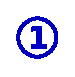
\includegraphics[scale=0.45]{images/1.eps}}, das sich in der Fenstermitte befindet. Darin wird der Globus, die Kartenebene oder eine Sonnensystemansicht angezeigt. Der sichtbare Kartenausschnitt kann interaktiv mit Maus oder Tastatur verschoben, gedreht gezoomt und gekippt werden.
	\item Am linken Rand des Fensters befindet sich die \textit{Seitenleiste} \index{Seitenleiste} \raisebox{-1pt}{
\includegraphics[scale=0.45]{images/2.eps}}, die die meisten Steuerungsoptionen bereitstellt. Der obere Teil ist in Tabs unterteilt, mit denen Funktionen gruppiert werden; der untere Teil zeigt Details zum momentan zentrierten Punkt an. Um den sichtbaren Kartenbereich zu vergrößern, ist sie ausblendbar.
	\item Am rechten Rand \raisebox{-1pt}{
\includegraphics[scale=0.45]{images/3.eps}} befindet sich ein Schieber, mit dem das Zoomlevel angezeigt und geändert werden kann.
	\item Die \textit{Statusleiste} \raisebox{-1pt}{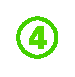
\includegraphics[scale=0.45]{images/4.eps}} am unteren Rand beinhaltet Informationen über den zentrierten Punkt, wie Koordinaten und Maßstab. Außerdem wird der Fortschritt im Hintergrund geladener Daten angezeigt.
\end{itemize}

\vspace{1cm}
\begin{figure}[!htb]
	\centering
	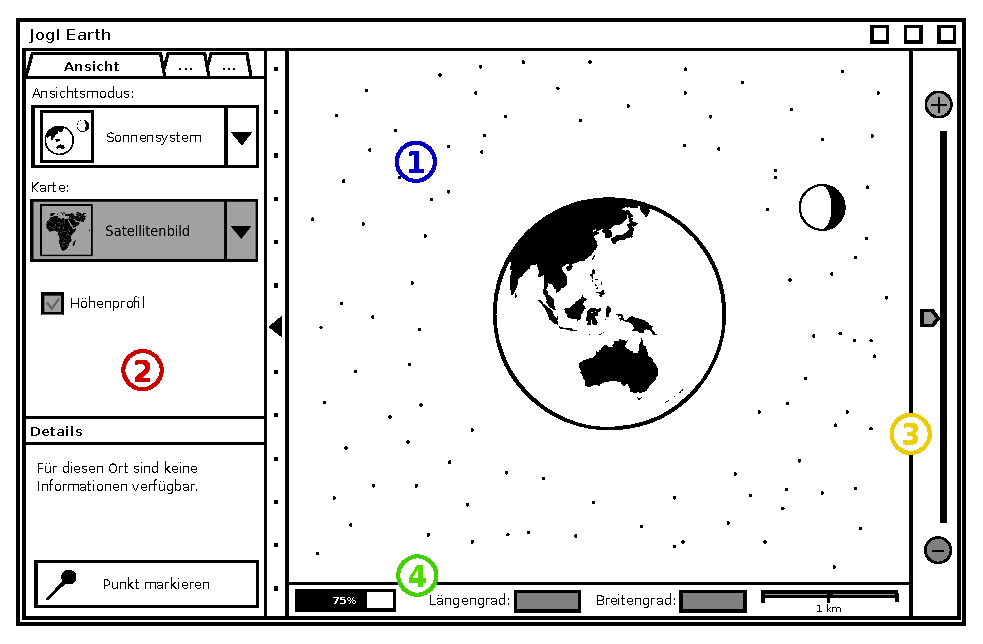
\includegraphics[scale=0.9]{GUI-Sonnensystem.eps}
	\caption{Die Benutzeroberfläche mit geöffnetem Ansichts-Tab im Sonnensystemmodus}
\end{figure}


\newpage
\vspace{3mm}
\subsection{Programm-Icons}
\vspace{2mm}
\begin{tabular}{|p{3cm}|p{10cm}|}
\hline 
\rule[-1ex]{0pt}{4ex} \textbf{Symbol} & \textbf{Erläuterung} \\ 
\hline
\hline
\rule[-1ex]{0pt}{4ex}  \parbox[c]{1em}{
\includegraphics[scale=0.6]{Logo-Print.eps}} &  Logo von \JoglEarth \\ 
\hline
\rule[-1ex]{0pt}{4ex}  \parbox[c]{1em}{
\includegraphics[scale=0.2]{Logo.eps}} & Programm-Icon \\ 
\hline
\rule[-1ex]{0pt}{4ex}  \parbox[c]{1em}{
\includegraphics[scale=1.4]{images/Hinzufugen.eps}} &  Stecknadel zum markieren eines Punktes \\ 
\hline
\rule[-1ex]{0pt}{4ex}  \parbox[c]{1em}{
\includegraphics[scale=1.4]{images/Entfernen.eps}} & Stecknadel zum entfernen eines Punktes \\ 
\hline
\rule[-1ex]{0pt}{4ex}  \parbox[c]{1em}{
\includegraphics[scale=1.7]{images/Zoom_plus.eps}} & Plus beim Zoomen \\ 
\hline
\rule[-1ex]{0pt}{4ex}  \parbox[c]{1em}{
\includegraphics[scale=1.7]{images/Zoom_minus.eps}} & Minus beim Zoomen \\ 
\hline
\rule[-1ex]{0pt}{4ex}  \parbox[c]{1em}{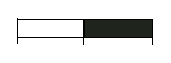
\includegraphics[scale=0.6]{images/Massstab.eps}} & Maßstab \\ 
\hline
\rule[-1ex]{0pt}{4ex}  \parbox[c]{1em}{
\includegraphics[scale=1.6]{images/Handbuch.eps}} &  Handbuch-Icon \\ 
\hline
\rule[-1ex]{0pt}{4ex}  \parbox[c]{1em}{
\includegraphics[scale=1.6]{images/infoButton.eps}} &  About-Icon \\ 
\hline
\end{tabular}


\newpage
\vspace{3mm}
\subsection{Navigation}

\vspace{3mm}
\subsubsection*{Mausbelegung}
\begin{tabular}{|>{\centering \arraybackslash}m{3cm}|m{10cm}|}
\hline

\includegraphics[scale=1.0]{images/mouseDrag_left.eps} & Drehen der Erdkugel / Verschieben der Karte \\ 
\hline 

\includegraphics[scale=1.0]{images/mouseDoubleClick_left.eps} & Punkt unter dem Mauszeiger im Kartenfenster zentrieren \\
\hline

\includegraphics[scale=1.0]{images/mouseDrag_right.eps} & Kippen der Kamera \\
\hline

\includegraphics[scale=1.0]{images/mouse_scrollen.eps} & Zoomen der Ansicht \\
\hline
\end{tabular} 


\vspace{3mm}
\subsubsection*{Tastaturbelegung}
\begin{tabular}{|>{\centering \arraybackslash}m{3cm}|m{10cm}|}
\hline
\rule[-1ex]{0pt}{7ex}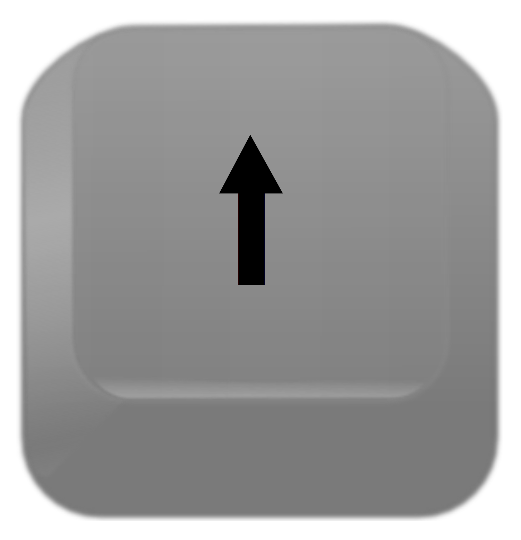
\includegraphics[scale=0.08]{images/key_arrow_up.eps}& \multirow{3}{*}{Drehen der Erdkugel / Verschieben der Karte}\\
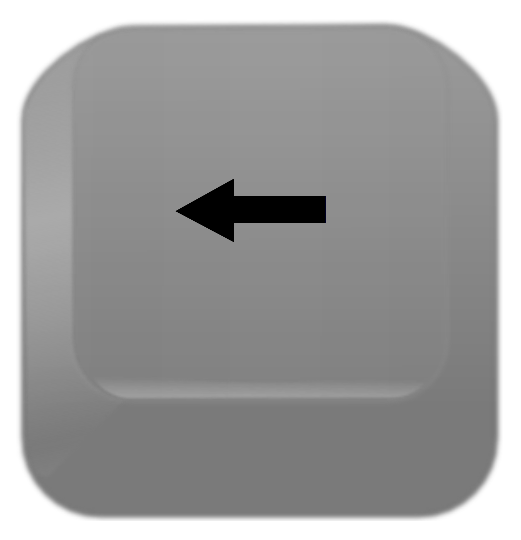
\includegraphics[scale=0.08] {images/key_arrow_left.eps} 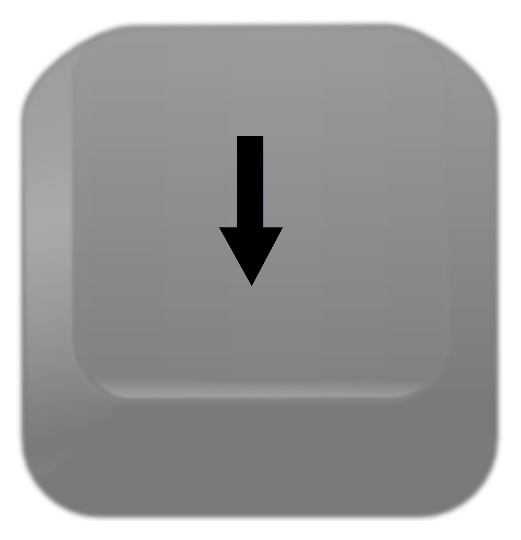
\includegraphics[scale=0.08]{images/key_arrow_down.eps} 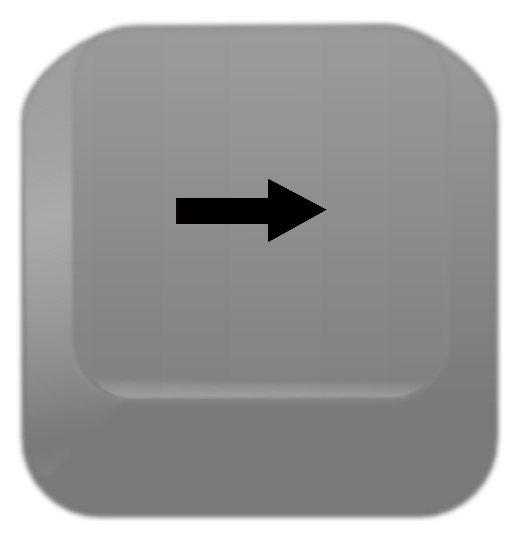
\includegraphics[scale=0.08]{images/key_arrow_right.eps} &  \\
\hline
\rule[-1ex]{0pt}{7ex} 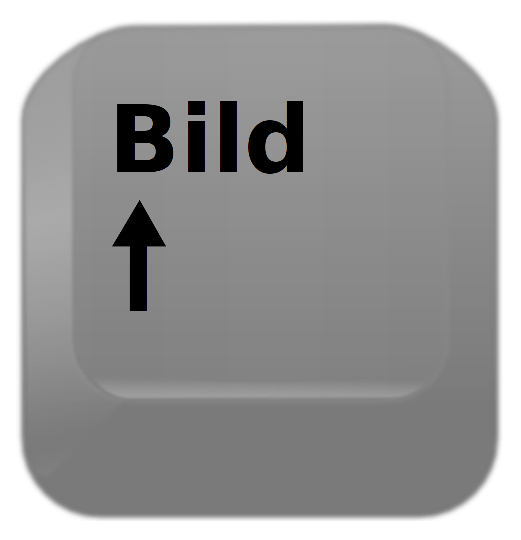
\includegraphics[scale=0.08]{images/key_Bild_Auf.eps}  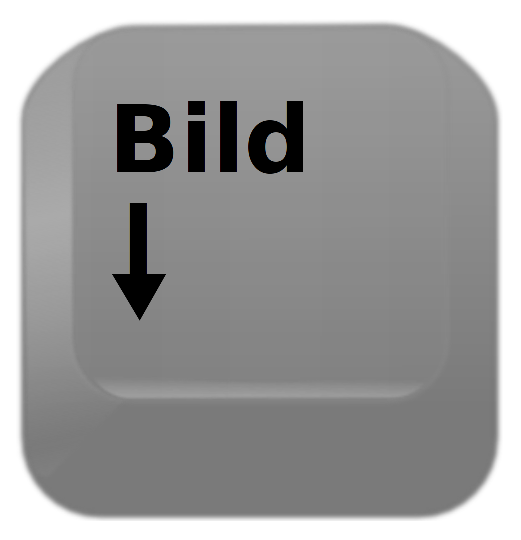
\includegraphics[scale=0.08]{images/key_Bild_Ab.eps} & Kippen der Kamera nach oben / unten\\
\hline
\rule[-1ex]{0pt}{7ex} 
\includegraphics[scale=0.08]{images/key_Pos1.eps} 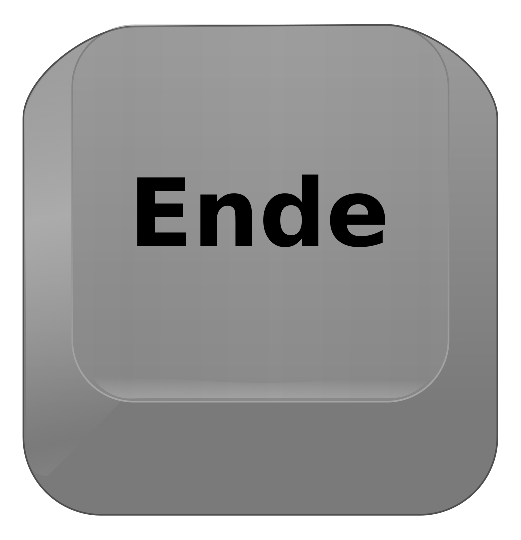
\includegraphics[scale=0.08]{images/key_Ende.eps} & Kippen der Kamera nach links / rechts \\
\hline
\rule[-1ex]{0pt}{7ex} 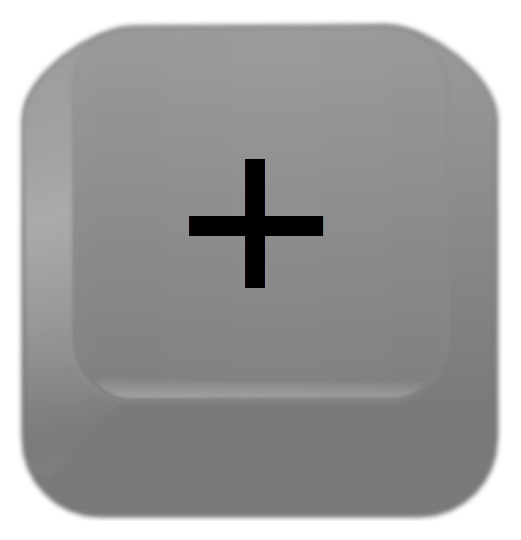
\includegraphics[scale=0.08]{images/key_Plus.eps}  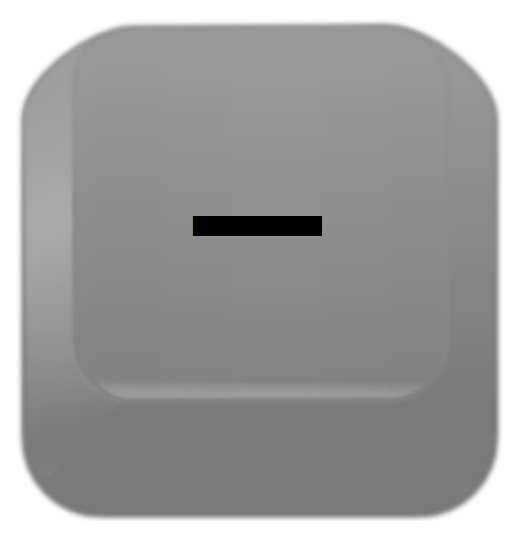
\includegraphics[scale=0.08]{images/key_Minus.eps} & Zoomen der Ansicht \\
\hline
\rule[-1ex]{0pt}{7ex} 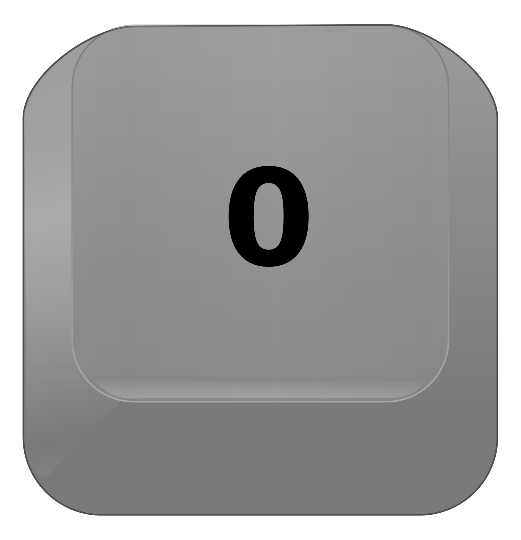
\includegraphics[scale=0.08]{images/key_0.eps} & Rücksetzen des Kippens \\ 
\hline
\rule[-1ex]{0pt}{7ex} 
\includegraphics[scale=0.08]{images/key_F1.eps} & Anzeige des Benutzerhandbuchs \\ 
\hline
\rule[-1ex]{0pt}{7ex} 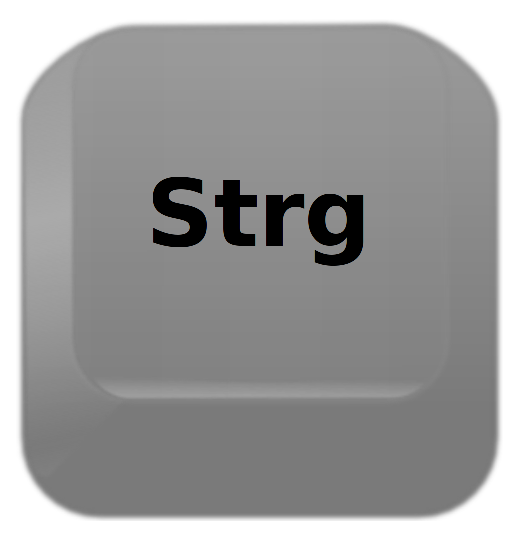
\includegraphics[scale=0.08]{images/key_Strg.eps} \rule[-1ex]{0pt}{7ex}\raisebox{0.7em}{\textbf{+}} 
\includegraphics[scale=0.08]{images/key_Q.eps} & Beenden der Anwendung \\ 
\hline
\end{tabular}


\vspace{3mm}
\section{Ansichtsmodi} \index{Ansichtsmodi}
\JoglEarth bietet zahlreiche Darstellungsmöglichkeiten für diverse Ansichten. Im folgenden werden die wählbaren Modi kurz erklärt.

\vspace{3mm}
\subsection{Sonnensystem} \index{Ansichtsmodi!Sonnensystem}
Diese Ansicht stellt ein detailliertes Modell von Sonne, Mond und Erde dar, wobei der Mond um die Erde kreist.

\vspace{3mm}
\begin{tabular}{>{\centering \arraybackslash}m{1cm} m{14cm}}

\includegraphics[scale=0.5]{images/info.eps} &  In dieser Ansicht können keine weiteren Funktionalitäten genutzt werden, wie beispielsweise Eingabe von Längen- oder Breitengrad, Ändern des Zoomlevels, Aktivieren des Höhenprofils, Markieren von Punkten.
\end{tabular}

%Screenshot


\vspace{3mm}
\subsection{Globus} \index{Ansichtsmodi!Globus}
Diese Ansicht visualisiert einen Globus, welcher die Anzeige von den unten gelisteten \textref{Kartentypen} unterstützt.

%Screenshot
\vspace{3mm}
\begin{tabular}{>{\centering \arraybackslash}m{1cm} m{14cm}}

\includegraphics[scale=0.5]{images/info.eps} &  \textbf{Navigation:} Der Globus kann gedreht, vergrößert, verkleinert und gekippt werden.
\end{tabular}

\vspace{3mm}
\begin{tabular}{>{\centering \arraybackslash}m{1cm} m{14cm}}

\includegraphics[scale=0.5]{images/info.eps} &  \textbf{Funktionalität:} Diese Ansicht unterstützt die gesamte Funktionalität von \JoglEarth , wie beispielsweise Aktivieren des Höhenprofils, Markieren von Punkten, etc.
\end{tabular}


\vspace{3mm}
\subsection{Karte} \index{Ansichtsmodi!Karte}
Diese Ansicht visualisiert eine Kartenebene, welche die Anzeige von den unten gelisteten \textref{Kartentypen} unterstützt.


%Screenshots
\vspace{3mm}
\begin{tabular}{>{\centering \arraybackslash}m{1cm} m{14cm}}

\includegraphics[scale=0.5]{images/info.eps} &  \textbf{Navigation:} Die Kartenebene kann gedreht, vergrößert, verkleinert und gekippt werden.
\end{tabular}

\vspace{3mm}
\begin{tabular}{>{\centering \arraybackslash}m{1cm} m{14cm}}

\includegraphics[scale=0.5]{images/info.eps} &  \textbf{Funktionalität:} Diese Ansicht unterstützt die gesamte Funktionalität von \JoglEarth , wie beispielsweise Aktivieren des Höhenprofils, Markieren von Punkten, etc.
\end{tabular}


\vspace{3mm}
\section{Kartentypen} \index{Kartentypen}
\JoglEarth bietet zahlreiche Kartentypen, die im folgenden näher betrachtet werden.

\vspace{3mm}
\subsection{Satellit} \index{Kartentypen!Satellit}
Unter diesem Kartentyp versteht man Satellitenbilder, welche Aufnahmen der Erdoberfläche aus der Perspektive eines Satelliten zeigen.
%Screenshot

\vspace{3mm}
\subsection{OpenStreetMap} \index{Kartentypen!OpenStreetMap}
\JoglEarth setzt auf die folgenden freien Kartenmaterialien des OpenStreetMap-Projekts, welche von den jeweiligen Servern zeitnahe geladen werden.

\begin{itemize}
\item Straßenkarte \index{OpenStreetMap!Straßenkarte}
\item Radkarte \index{OpenStreetMap!Radkarte}
\item Pistenkarte \index{OpenStreetMap!Pistenkarte}
\item Wander- und Reitkarte \index{OpenStreetMap!Wander- und Reitkarte}
\item OSM2World \index{OpenStreetMap!OSM2World}
\end{itemize}

\vspace{3mm}
\subsection{Kinderweltkarte} \index{Kartentypen!Kinderweltkarte}


\vspace{3mm}
\begin{tabular}{>{\centering \arraybackslash}m{1cm} m{14cm}}

\includegraphics[scale=0.5]{images/quest.eps} &  Versuchen Sie sich durch die Ansichten und Kartentypen zu navigieren.
\end{tabular}



\vspace{3mm}
\section{Standard-Einstellungen}
Bei erstmaligem Starten von \JoglEarth sind standardmäßig folgende Einstellungen gesetzt:

\begin{itemize}
\item Ansichtsmodus: Sonnensystem
\item Kartentyp: -
\item Höhenprofil: deaktiviert
\item Zoomlevel: 50%
\item Overlays: alle deaktiviert
\item Sprache: Deutsch
\item Grafikeinstellungen:
	\begin{itemize}
	\item Antialiasing: aus
	\item Detailgrad: niedrig
	\end{itemize}
\item Cachegrößen:
	\begin{itemize}
	\item Arbeitsspeicher: 50 MB
	\item Dateisystem: 100 MB
	\end{itemize}
\end{itemize}














\chapter{Funktionen}
%inkl. Übungsaufgaben/ Szenarien, wie was funktioniert Wichtig: Tipps \& Tricks nennen


\section{Sprache der Benutzeroberfläche}
Einstellen der Benutzeroberfläche \index{Benutzeroberfläche}:


\vspace{3mm}
\section{Höhenprofil}
\index{Höhenprofil}
Die Höhenprofile werden anhand von NASA \index{NASA} SRTM \index{SRTM} Daten ermittelt.

\vspace{3mm}
\begin{tabular}{>{\centering \arraybackslash}m{1cm} m{14cm}}

\includegraphics[scale=0.5]{images/info.eps} &  Zur optimalen Darstellung des Höhenprofils empfiehlt sich Zoomlevel ... \\ 
\end{tabular} 


\vspace{3mm}
\section{Eingabe von Längen- und Breitengraden}

\vspace{3mm}
\section{Ändern des Zoomlevels}

\vspace{3mm}
\section{Markierungen setzen}

\vspace{3mm}
\section{Benutzermarkierungen}
Das Feld der Benutzermarkierungen befindet sich im Orte-Tab.
Übung: Markierungen einblenden / ausblenden

\vspace{3mm}
\section{Markierungen entfernen}

\vspace{3mm}
\section{Suchfunkion}
Die Suchfunktion wird über Nominatim ausgeführt. Bei den Suchanfragen ist ein Limit gesetzt. Wundern Sie sich daher nicht, wenn ein gesuchter Ort nicht gefunden werden kann. \\

\vspace{3mm}
\begin{tabular}{>{\centering \arraybackslash}m{1cm} m{14cm}}

\includegraphics[scale=0.5]{images/info.eps} &  Die Suchbegriffe werden von links nach rechts (vom Speziellen zum Allgemeinen) abgearbeitet und dann von rechts nach links, wenn das fehlschlägt. \\ 
\end{tabular} 

\vspace{3mm}
Beispiele: \textit{Brandenburger Tor, Berlin} als auch \textit{Berlin, Brandenburger Tor} wird ein Ergebnis liefern.\\

\vspace{3mm}
\begin{tabular}{>{\centering \arraybackslash}m{1cm} m{14cm}}

\includegraphics[scale=0.5]{images/info.eps} &  Kommas sind nicht notwendig, verbessern aber die Suchgeschwindigkeit durch Reduzierung der Komplexität der Suchanfrage.  \\ 
\end{tabular} 

\vspace{3mm}
Beispiel:
Es wird auch nachfolgende Abfrage funktionieren: \textit{Brandenburger Tor Berlin}

Die Suchergebnisse werden im Orte-Tab angezeigt.
Übung: Suche Passau...

\vspace{3mm}
\section{POIs} \index{POIs}
\subsection*{Liste der POIs}
Bei der Qualität des Detailgrads der POIs baut \JoglEarth auf die Datenpflege der OverpassAPI. Inwieweit die Daten konsistent geführt werden kann im Rahmen dieses Projekts nicht beeinflusst werden. Es werden keinerlei Ergänzungen, Fehlerkorrekturen oder Ähnliches an den  Antworten der OverpassAPI vorgenommen.\\

\vspace{3mm}
\begin{tabular}{|p{3cm}|p{10cm}|}
\hline 
\rule[-1ex]{0pt}{4ex} \textbf{Symbol} & \textbf{Erläuterung} \\ 
\hline
\hline
\rule[-1ex]{0pt}{4ex}  \parbox[c]{1em}{
\includegraphics[scale=1.6]{images/POI_Shop.eps}} &  SHOPS \\ 
\hline
\rule[-1ex]{0pt}{4ex}  \parbox[c]{1em}{
\includegraphics[scale=1.6]{images/POI_Restaurant.eps}} & RESTAURANTS \\ 
\hline
\rule[-1ex]{0pt}{4ex}  \parbox[c]{1em}{
\includegraphics[scale=1.6]{images/POI_nightlife.eps}} &  NIGHTLIFE \\ 
\hline
\rule[-1ex]{0pt}{4ex}  \parbox[c]{1em}{\includegraphics[scale=1.6]{images/POI_Bank.eps}} & BANK \\ 
\hline
\rule[-1ex]{0pt}{4ex}  \parbox[c]{1em}{\includegraphics[scale=1.6]{images/POI_Toilets.eps}} & TOILETS \\ 
\hline
\rule[-1ex]{0pt}{4ex}  \parbox[c]{1em}{\includegraphics[scale=1.6]{images/POI_Grocery.eps}} & GROCERY \\ 
\hline
\rule[-1ex]{0pt}{4ex}  \parbox[c]{1em}{\includegraphics[scale=1.6]{images/POI_Activity.eps}} & ACTIVITY \\ 
\hline
\rule[-1ex]{0pt}{4ex}  \parbox[c]{1em}{\includegraphics[scale=1.6]{images/POI_hiking_cycling.eps}} & HIKING\_CYCLING \\ 
\hline
\rule[-1ex]{0pt}{4ex}  \parbox[c]{1em}{\includegraphics[scale=1.6]{images/POI_education.eps}} &  EDUCATION \\ 
\hline
\rule[-1ex]{0pt}{4ex}  \parbox[c]{1em}{\includegraphics[scale=1.6]{images/POI_health.eps}} &  HEALTH \\ 
\hline
\rule[-1ex]{0pt}{4ex}  \parbox[c]{1em}{\includegraphics[scale=1.6]{images/POI_post.eps}} &  POST \\ 
\hline
\rule[-1ex]{0pt}{4ex}  \parbox[c]{1em}{\includegraphics[scale=1.6]{images/POI_hotels.eps}} &  HOTELS \\ 
\hline
\end{tabular}

Übung: POIs einblenden / ausblenden





\vspace{3mm}
\section{Grafikeinstellungen}

\vspace{3mm}
\subsection{Antialiasing} \index{Antialiasing}

\vspace{3mm}
\subsection{Detaillevel} \index{Detaillevel}




\vspace{3mm}
\section{Cachegrößen} \index{Cachegrößen}

\vspace{3mm}
\subsection{Arbeitsspeicher}

\vspace{3mm}
\subsection{Dateisystem}









\chapter{Datenorganisation}

% Wo werden die Daten gespeichert. Im MemoryCache und FileSystemCache.
% Welche Benutzereinstellungen werden in Settings gespeichert - Tabelle machen
% Vom Benutzer markierte Punkte werden gespeichert.

\section{Speicherung Kartendaten \& Benutzermarkierungen}
% Bildchen einfügen, welches zeigt, wo die Daten auf der Festplatte gespeichert werden

Während der Nutzung von \JoglEarth werden die benötigten Kartendaten und die vorgenommenen Benutzermarkierungen zu deren Wiederverwendung in die verfügbaren Caches geschrieben. Das sind
\begin{itemize}
\item OpenStreetMap Kartenmaterialien
\item SRTM Höhendaten
\item Benutzermarkierungen
\end{itemize}



\vspace{3mm}
\section{Settings}
% Welche Settings werden gespeichert. Grafische Darstellung

\vspace{3mm}
\subsection*{Einstellungen:}
Folgende getätigte Einstellungen werden bei ordnungsgemäßer Programmbeendigung gespeichert:
\begin{itemize}
\item Ansichtsmodus
\item Kartentyp
\item Höhenprofil
\item Sprache
\item Grafikeinstellungen:
	\begin{itemize}
	\item Detailgrad
	\end{itemize}
\item Cachegrößen
	\begin{itemize}
	\item Arbeitsspeicher
	\item Dateisystem
	\end{itemize}
\end{itemize}




\cleardoublepage
\addcontentsline{toc}{chapter}{\indexname}
\printindex


\end{document}